\section{ Sentiment Analysis Methods }
To the best of our knowledge we have evaluated certain popular approaches in solving the problem of extracting latent sentiment in a media content. The sentiment analysis methods broadly fall into two bins. One is the Content based Image retrieval (CBIR) \cite{CBIRSurvey} set of approaches, which actually analyse the image structure and contents to extract features and inferences about the image. The second bin is emotional semantic image retrieval (ESIR) \cite{ESIRSurvey} which aim at trying to extract the semantic gist of a particular image. Human brain is great at extracting such semantics. For example it is very natural for a person to describe a particular image as "picturesque" or "scenic" or to describe someone's clothing as "tacky" , "classy" or "elegant". These semantic classes, no matter how subjective, are also sufficiently descriptive for another human being to process. 
In the subsections to come, we will discuss some of the popular perceptual sentiment analysis methods.

%\subsection{ SENTIBANK }
%Sentibank \cite{SentiBank} is a method that proposes a Visual Sentiment Ontological approach towards image perceptual sentiment retrieval. The method tries to match an image with an Adjective noun pairs which give a visual ontology about the structure of an image. The pairs are extracted using trained detectors which train on a dataset acquired from Flickr images. The adjective noun pair concept labels are verified using Mechanical Turk. The result is 

\subsection{Facial Action Coding System (FACS) based methods:}
Facial Action Coding System (FACS) based approach towards understanding human affects was the pioneering research done at CMU that paved the way of modern affective computing. The paper \cite{670980} talks about this pioneering research. The method works on a very important base of Facial Action Coding \cite{FACS} system which encodes movement of specific muscles of human face and encodes actions units as a combinations of one or more of these movements. These AUs or Action Units are then carefully measured from frontal images of faces and then models are built on top of these measurements to classify different emotions.  

\begin{figure}
\centering
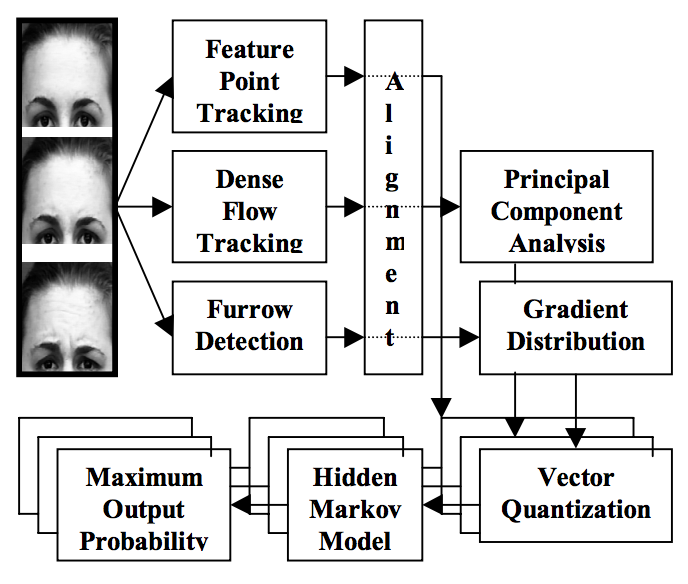
\includegraphics[width=\columnwidth]{figures/FAU_Kanade}
\caption{\textbf{System architecture of FACS AU based Emotion recognition}}
\label{fig:FACSAU}
\end{figure}

The paper evaluates these AU based methods for specific AUs. They do not show a very convincing performance analysis for the 7 prime emotion bins, but evaluate classification accuracy for each of the AUs. The performance shows very promising accuracy for detecting AUs in upper and lower part of the face. Works like \cite{1027968} \cite{5771366} take these concepts forward and use features in AU zones to build classifiers. These studies employ features like Pyramids of Histograms of Gradients (PHOG) and Local Phase Quantisation (LPQ) to classify across 5 key emotions of anger, fear, joy, relief and sadness. Their methods attain a very impressive performance bracket of 67 to 74 percent detection accuracy.

\subsection{ Semi-supervised learning models }
Over the past two decades, with the surprising developments parallel computing and general purpose graphics processor computing, the space for scaling up and parallelising sparse computation has increased exponentially. This paved the way for extremely fast and scalable neural network frameworks. 